\section{FS Track Protocol}

    Para que o serviço funcione devidamente, o \textit{tracker} tem de conhecer todos os blocos de cada cliente e transmitir essa informação sempre que necessário, perante isto é necessário definir um protocolo de comunicação que sirva esse propósito.

    As mensagens trocadas com o \textit{tracker} seguem quase todas uma estrutura bem definida, na qual se associam endereços IP (clientes) a blocos de ficheiros, como tal optámos por criar um segmento designado de \textit{TCPPacket} que representa o formato das mensagens passadas ao \textit{tracker}.

    \begin{figure}[hb!]
        \centering
        \includegraphics[width=0.45\textwidth]{Imagens/Headers/tracker.png}
        \caption{Cabeçalho de um \textit{TCPPacket}}
    \end{figure}
    \vspace{-10pt}

    A princípio pensámos que seria um erro misturar informações de \textit{layers} diferentes no cabeçalho do segmento, contudo concluímos que assim teríamos uma maior flexibilidade ao manipular e controlar os \textit{sockets} que conectam os clientes ao \textit{tracker}.

    \subsection{Protocolo}

        Este campo tem como objetivo identificar a função de um \textit{TCPPacket}, como tal existem múltiplos valores à sua disposição, sendo que cada um exige um tratamento diferente da informação do segmento. Além disso, convém realçar que o cliente e o \textit{tracker} não podem aplicar as mesmas opções nas suas mensagens. 

        \begin{itemize}

            \item \textbf{Enviado pelo cliente}
                
            \begin{itemize}
                
                \item \textbf{HELLO:} É enviado no momento em que o cliente anuncia os seus ficheiros ao \textit{tracker}. 
    
                \item \textbf{GET:} Serve para obter uma listagem dos endereços IP associados a um determinado ficheiro. 
    
                \item \textbf{EXIT:} Indica a intenção do cliente abandonar a rede.
            
            \end{itemize}

            \newpage
            \item \textbf{Enviado pelo \textit{tracker}}

            \begin{itemize}
                
                \item \textbf{HELLOACK:} Confirma a receção da informação dos ficheiros de um cliente.

                \item \textbf{GETACK:} Envia a listagem de endereços IP associados ao ficheiro requerido pelo cliente.

                \item \textbf{EXITACK:} Confirma que os dados do cliente foram removidos da estrutura central de dados.

                \item \textbf{ACK:} Confirma a receção de outras quaisquer mensagens.
            
            \end{itemize}
            
        \end{itemize}

    \subsection{Dados}

        Dentro deste campo podem ser inseridos dois tipos de mensagens, uma é especialmente dirigida ao cliente, enquanto que a outra tem como destinatário o \textit{tracker}, consequentemente nunca podem ser utilizadas em conjunto no mesmo segmento.

        Se abstrairmos um pouco o pensamento, reparamos que o cliente comunica sempre do mesmo modo com o \textit{tracker}, independentemente do protocolo que aplica nos seus segmentos. As mensagens resumem-se a uma lista de ficheiros com os respetivos blocos, sendo que para \textit{GET} é enviada uma lista de ficheiros sem blocos, enquanto que para \textit{EXIT} a lista assume-se como vazia.

        Ao aplicarmos o mesmo raciocínio às mensagens enviadas a partir do \textit{tracker}, concluímos que as mesmas correspondem a uma lista de blocos com os respetivos endereços IP.

        \begin{center}
            
            \textit{ToTracker} = \textit{[(Ficheiro,[Bloco])]} 
            
            \textit{ToClient} = \textit{[(Bloco,[Endereço IP])]}
        
        \end{center}

    \subsection{Funcionamento}

        Estando o segmento \textit{TCPPacket} totalmente especificado e conhecendo o comportamento do \textit{tracker} face às mensagens que recebe do cliente, podemos traçar aquilo que seria o fluxo normal da comunicação entre o \textit{tracker} e o cliente.

        \begin{enumerate}
            
            \item O cliente lê todos os ficheiros que tem na sua pasta partilhada e procede à divisão em blocos dos mesmos.

            \item O cliente organiza a informa num \textit{TCPPacket} cujo protocolo corresponde a \textit{HELLO}, e envia ao \textit{tracker}.

            \item O \textit{tracker} recebe o segmento e insere a informação que este contem numa estrutura central de dados.

            \item O \textit{tracker} envia um \textit{TCPPacket} com protocolo \textit{HELLOACK} ao cliente.

            \item O cliente recebe o \textit{HELLOACK} e percebe que daí em diante pode ser contactado por outros clientes.

            \item O cliente deseja transferir o ficheiro \textit{A}, como tal envia um \textit{GET ficheiro A} ao \textit{tracker}.

            \item O \textit{tracker} recebe o segmento e recolhe todos os endereços IP associados ao \textit{ficheiro A}.

            \item O \textit{tracker} envia um \textit{GETACK} com a informação necessária para contactar os restantes clientes.

            \item O cliente recebe o segmento e inicia a comunicação com os restantes a fim de obter o ficheiro.

            \item O cliente pretende abandonar a rede, para isso envia um \textit{EXIT}.

            \item O \textit{tracker} recebe o segmento e procede à eliminação de toda a informação relativa ao cliente.
            
            \item O cliente deixa de constar na estrutura central do \textit{tracker}, como tal é enviado um \textit{EXITACK}.

            \item O cliente recebe o segmento e fecha o \textit{socket}. 

        \end{enumerate}

        \begin{figure}[hb!]
            \centering
            \includegraphics[width=0.75\textwidth]{Imagens/Diagramas Temporais/tracker.png}
            \caption{Diagrama temporal da comunicação entre o \textit{tracker} e o cliente}
        \end{figure}

    \subsection{Estruturas de Dados}

        No momento em que um cliente se anuncia à rede, este partilha as informações dos seus ficheiros com o \textit{tracker}, como tal é necessária uma estrutura de dados robusta que permita efetuar consultas em tempo constante dos endereços IP associados a determinados blocos.

        A estrutura mais adequada para este problema resulta do encadeamento de dois \textit{HashMap's}, sendo que o primeiro mapeia um ficheiro para um \textit{map} de blocos, enquanto que o segundo mapeia um bloco para uma lista de endereços IP.

        Já em relação ao cliente, este não necessita de qualquer estrutura minimamente complexa, visto que o seu comportamento baseia-se na leitura de ficheiros e no envio/receção de segmentos.

        \begin{figure}[hb!]
            \centering
            \includegraphics[width=0.85\textwidth]{Imagens/Estruturas/map.png}
            \caption{Esquema da estrutura de dados do \textit{tracker}}
            \label{fig:enter-label}
        \end{figure}